\documentclass{standalone}
\usepackage{tikz}

\usetikzlibrary{calc,math}


\begin{document}

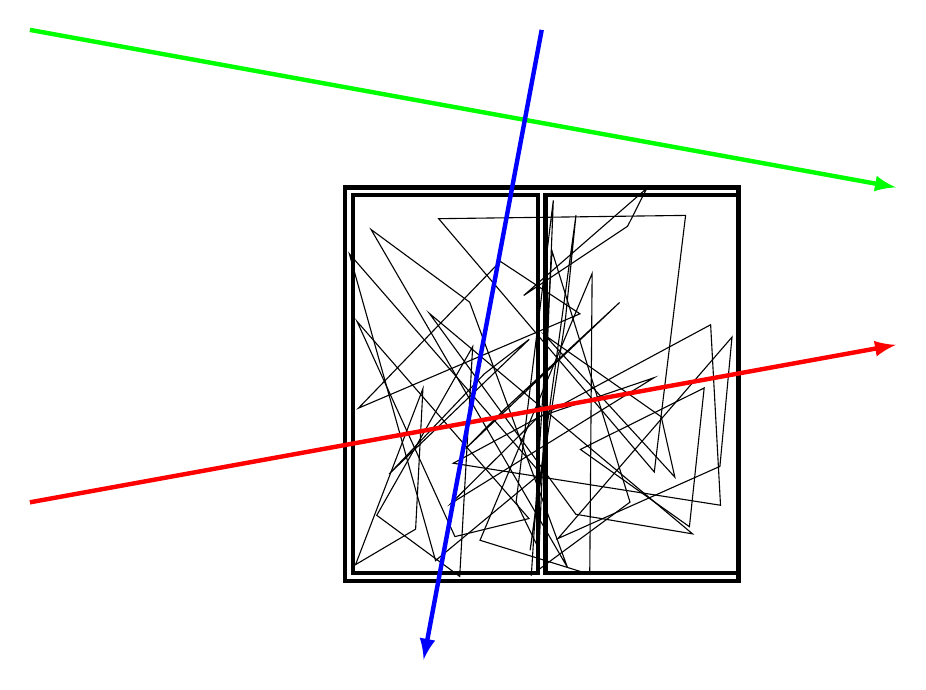
\begin{tikzpicture}
  \draw[ultra thick] (0,0) rectangle (5,5);
  \draw[ultra thick] (0.1,0.1) rectangle (2.45,4.9);
  \draw[ultra thick] (2.55,0.1) rectangle (5,4.9);

  \foreach \i in {1,...,20} {
    \tikzmath{
      real \ax;
      real \ay;
      real \bx;
      real \by;
      real \cx;
      real \cy;
      \ax=random() * 5;
      \ay=random() * 5;
      \bx=random() * 5;
      \by=random() * 5;
      \cx=random() * 5;
      \cy=random() * 5;
    }

    \draw (\ax,\ay) -- (\bx,\by) -- (\cx,\cy) -- cycle;
  }

  \draw[ultra thick,green,-latex] (-4,7) -- (7,5);
  \draw[ultra thick,red,-latex] (-4,1) -- (7,3);
  \draw[ultra thick,blue,-latex] (2.5,7) -- (1,-1);
\end{tikzpicture}

\end{document}